\section{Easy UnpackMe}
\begin{enumerate}
\item IDA直接打开,查看函数列表,只有一个start函数 \\
\item 双击 查看函数 ,开始分析\\
\item 空格 切换为Graph视图 \\
\item 函数尾部跳出所有循环开始分析,查找到jmp语句:\lstinline$jmp     loc_401150$ \\
	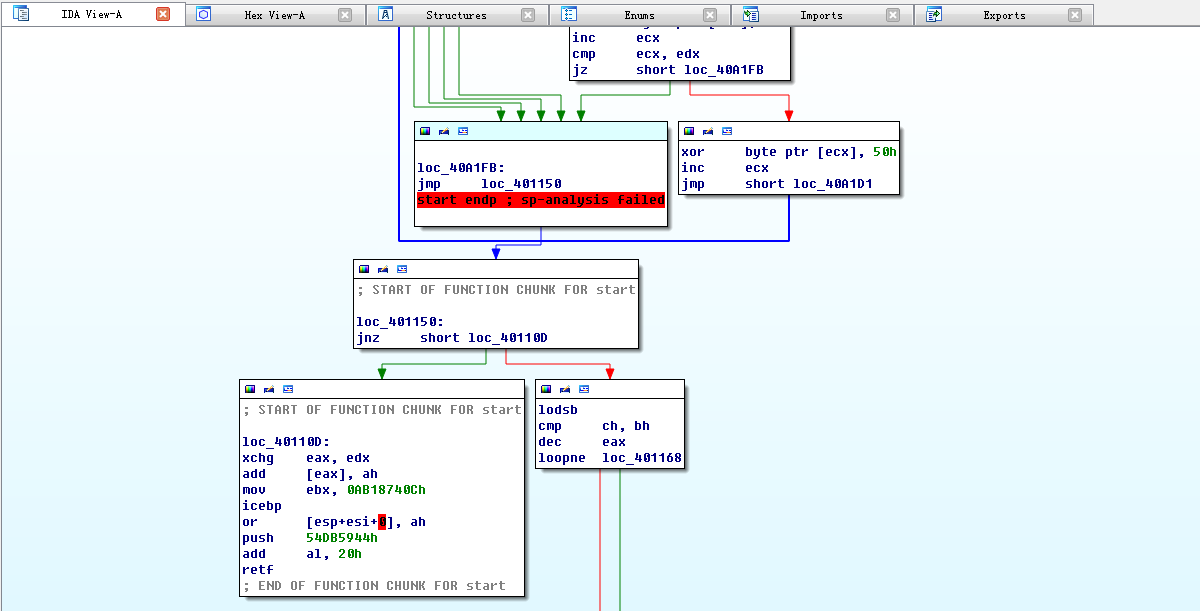
\includegraphics[width=10cm]{easyunpack-jmp} \\
	空格 切换为文本视图 \\
	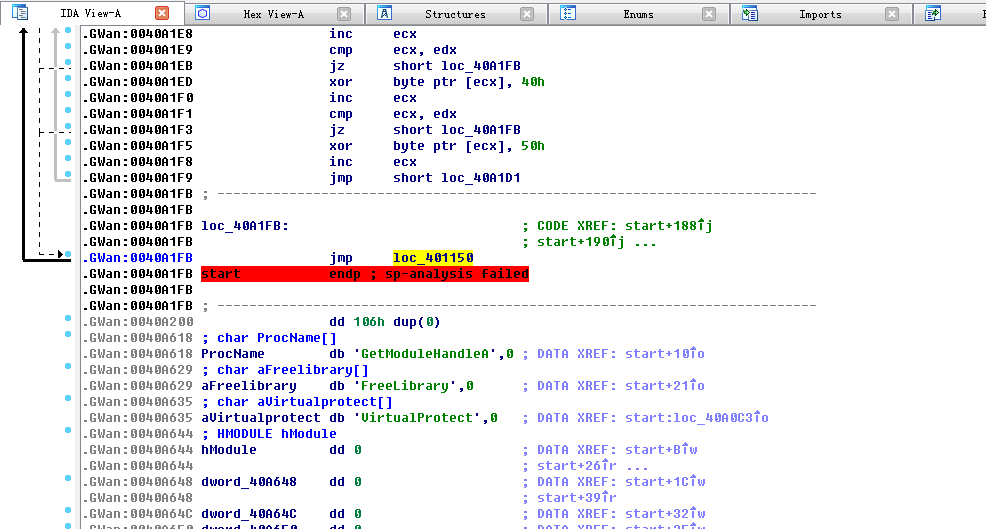
\includegraphics[width=10cm]{easyunpack-textjmp} \\
	双击\lstinline$loc_401150$ 跳转至定义,查看地址得到:00401150 \\
	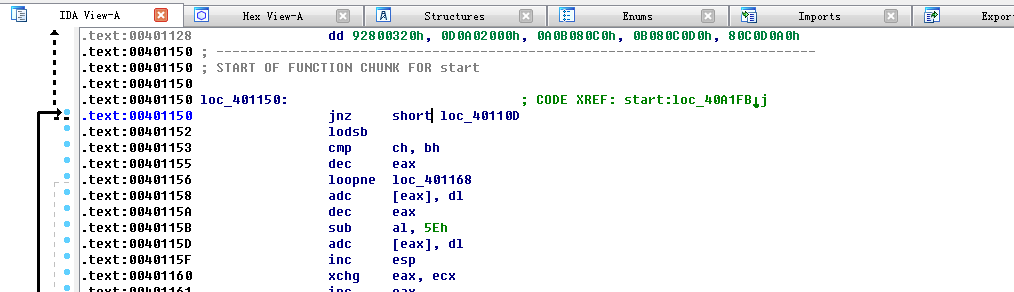
\includegraphics[width=10cm]{easyunpack-addr} \\
	flag : ``00401150''
\end{enumerate}